% Nature Sustainability Article - Governance, Competition and Procurement Decarbonization
% Format: Article (original research)
% Constraints: <=10 word title, <=150 word abstract, ~5,000 word main text, <=6 display items
% REVISED: Complete structural rewrite - Decarbonization Dead Zones framing

\documentclass[11pt,a4paper]{article}
\usepackage[T1]{fontenc}
\usepackage[utf8]{inputenc}
\usepackage[margin=1in]{geometry}
\usepackage{graphicx}
\usepackage{amsmath}
\usepackage{amssymb}
\usepackage[hypertexnames=false]{hyperref}
\usepackage{xurl}
\usepackage{booktabs}
\usepackage{float}
\usepackage{xcolor}
\usepackage{textcomp}
\usepackage{lineno}
\usepackage{setspace}
\usepackage{enumitem}
\usepackage{tabularx}
\usepackage{multirow}
\usepackage{longtable}
\usepackage{colortbl}

\linenumbers
\onehalfspacing
\renewcommand{\arraystretch}{1.12}

\newcommand{\tabnotes}[1]{%
	\par\vspace{0.45em}%
	\begin{minipage}{0.98\linewidth}
	\footnotesize\raggedright\textit{Notes:} #1
	\end{minipage}\par
}

% Graphics path for figures - look in Main_Figures subdirectory
\graphicspath{{Main_Figures/}{Extended_Data_Figures/}{figures/}}

% Title (9 words -- within Nature Sustainability's <=10-word limit)
\title{\Large\textbf{Governance Reform Unlocks Decarbonization Dead Zones in Public Procurement}}

\author{Abduxoliq Ashuraliyev$^{1,*}$}

\date{}

\begin{document}

\maketitle

\vspace{-0.5cm}
\noindent\rule{\textwidth}{0.5pt}

\begin{center}
$^{1}$Independent Researcher, Open Data Initiative, Tashkent, Uzbekistan

$^{*}$Corresponding author: Abduxoliq Ashuraliyev (jack00040008@outlook.com)

ORCID: 0009-0003-5482-5526
\end{center}

\noindent\vspace{0.3cm}

% Abstract (<=150 words as required by Nature Sustainability)
\begin{abstract}
\noindent Green public procurement can cut emissions only when buyers have real supplier choice. Using 21.6 million government contracts from 27 countries, we identify 22 ``Decarbonization Dead Zones'' where high carbon intensity and high single-bidder rates place \texteuro190--250 billion of annual EU spending beyond effective green criteria. In Europe, transparency reform appears to make high-carbon markets contestable: Directive 2014/24/EU is associated with a $-7.2$ percentage-point fall in single-bidder rates, reproduced at $-8.6$ pp ($p = 0.012$) using purely within-EU timing variation with zero external controls; the EU disclosure threshold increases bidder counts by $+0.32$ additional bidders; and the allocative channel is corroborated across facility-, sector-, and supplier-level data, including a 43\% within-sector EU ETS emissions gap, direct E-PRTR facility matching confirming $+65.3\%$ higher reported CO\textsubscript{2} in single-bidder contracts, and 2,327 EU SBTi-validated firms in Dead Zone sectors. Before governments can buy green, they must first make high-carbon markets contestable.
\end{abstract}

\noindent\textbf{Keywords:} green public procurement; governance; decarbonization dead zones; single-bidding; carbon intensity; difference-in-differences; regression discontinuity; supply chains

\vspace{0.5cm}
\noindent\rule{\textwidth}{0.5pt}

%----------------------------------------------------------------------
% Introduction (no section heading per Nature format)
%----------------------------------------------------------------------

At over \texteuro2 trillion annually in the EU alone---and approximately US\$10.4 trillion across the G20\cite{oecd2023procurement}---public procurement is one of the largest discretionary levers governments possess over private-sector supply chains\cite{oecd2024greenprocurement}. Green Public Procurement (GPP) programmes attempt to direct this spending toward lower-carbon suppliers---but GPP can only function where governments have a genuine choice. A contract awarded to the sole available supplier forecloses any environmental conditionality; a buyer cannot select a greener alternative when none exists. Despite this structural prerequisite, no study has systematically quantified where and why competition fails in high-carbon procurement, or measured the carbon cost of that failure at scale. Before governments can buy green, they must first make high-carbon markets contestable.

We use the term \textit{Decarbonization Dead Zones} as an operational label for procurement sectors that combine high carbon intensity with high single-bidder rates, i.e. markets where GPP has limited leverage because supplier choice is weak. Mapping 75 procurement sectors across 21.6 million contracts in 27 countries (2012--2023), we identify 22 sectors under global thresholds (6 under a stricter EU-context screen; SI Table~S18), together representing 51.5\% of procurement value. The concept is intended as a policy screen for contestability constraints in carbon-intensive procurement, not as a claim that these sectors form a natural or immutable class.

Critically, the competition--carbon relationship is governance-contingent, not universal. In EU-context countries with transparent procurement frameworks, competitive contracts encompass \textit{higher}-carbon procurement categories than single-bidder awards, producing a $-4.3\%$ negative premium\cite{eu2014directive}. We interpret this pattern as consistent with governance regimes in which higher-carbon sectors are more often procured competitively, creating the market conditions under which GPP can operate. In weaker institutional settings, the same sectors are more likely to remain single-sourced. This governance split, with $I^2 = 99.3\%$ cross-country heterogeneity, offers a candidate explanation for why GPP performance varies across institutional contexts\cite{grandia2015implementing,cheng2018green,ortegacarrasco2025gpp}. Non-European evidence is used as descriptive corroboration; the primary causal identification is European.

We therefore test whether EU procurement governance reform is associated with lower single-bidder rates. In a staggered Callaway \& Sant'Anna design, Directive 2014/24/EU is associated with a $-7.2$ percentage-point reduction in single-bidder rates (RMSPE permutation $p = 0.042$, rank 1 of 24). The result does not depend on external controls: a not-yet-treated C\&S specification using only within-EU transposition timing yields ATT $= -8.6$ pp ($p = 0.012$) with zero external comparators, leave-one-out bounds retain a $-4.75$ to $-8.46$ pp envelope, and a CanadaBuys proxy-control gives the same negative sign outside the EEA/TED panel. Rambachan \& Roth (2023)\cite{rambachan2023} sensitivity implies post-treatment parallel-trend violations would need to be $1.54{\times}$ larger than the worst pre-period first difference to explain the estimate away. A country-level dose-response falsification points the same way: higher 2012--2015 baseline single-bidder exposure predicts larger 2017--2019 declines ($r = -0.56$, $p = 0.0029$), whereas the analogous pre-treatment placebo is null ($r = 0.065$, $p = 0.75$; Fisher $z$ contrast $p = 0.018$).

The carbon interpretation is likewise bounded. The headline $-4.3\%$ premium is an EXIOBASE allocative portfolio measure, not a direct realized-emissions estimate. Independent checks test whether this allocative channel is visible in measured data: Eurostat shows the single- versus multi-bidder carbon gap narrowing by 66\% after reform ($p < 0.001$), EU ETS installation data show a 43\% P25-versus-median within-sector emissions gap across 195,603 facility-years ($d = -0.37$), annual E-PRTR matching links 10,804 procurement contract-years to reported facility CO\textsubscript{2}, within-supplier comparisons remain negative across 39,410 firms, and competition increases access to SBTi-validated suppliers from 0.82\% to 4.04\% in construction and from 1.16\% to 5.68\% in medical and pharmaceutical procurement. These results support governance reform as a first-stage condition for effective GPP in structurally thin markets, while leaving realized abatement as a downstream policy quantity.

These empirical blocks serve different inferential roles. The Dead Zone map is descriptive, the DiD and RDD identify competition responses, the Eurostat/EU ETS/E-PRTR/within-supplier/SBTi evidence tests whether the decarbonization interpretation survives independent measurement, and the later Monopoly Tax and Green Premium calculations are calibrated downstream implications rather than additional causal estimates.

\section{Results}

\subsection{The Carbon-Competition Gap: Aggregate Evidence}

Across 21.6 million government contracts from 27 countries (2012--2023), we find that the competition--carbon relationship is governance-contingent, not universal (Table~\ref{tab:ucurve}). Throughout, we define the ``single-bidder premium'' as the percentage difference in portfolio carbon intensity between single-bidder and multi-bidder contracts; a \textit{negative} premium indicates that single-bidder contracts concentrate in \textit{lower}-carbon sectors---the signature of governance reforms having opened high-carbon markets to competition. In the 26 EU-context countries with transparent procurement frameworks ($N = 13{,}638{,}933$), single-bidder contracts exhibit \textit{lower} portfolio carbon intensity than competitive awards: $-4.3\%$ ($t = -110$; Cohen's $d = -0.08$). With 13.6 million observations, all point estimates are statistically precise (95\% CIs $<\pm0.2$ pp); practical significance is assessed through effect sizes and policy-relevant benchmarks. The $d = -0.08$ is small per contract, but it operates across \texteuro190--250 billion in annual spending where the policy-relevant quantity is the aggregate sectoral allocation, not the individual contract effect---comparable in scale to the 3--5\% emission reductions attributed to carbon pricing in early-adoption EU ETS sectors\cite{herre2023emission}.

This negative premium---more pronounced for large contracts ($-7.8\%$; $d = -0.13$) than small ($-2.8\%$; $d = -0.05$)---indicates that governance reforms have opened the highest-carbon procurement sectors to competitive bidding. A model-free decile check identifies the remaining lock-in pockets: among the highest-carbon contracts (top decile), 13.9\% are single-bidder awards compared with 6.2\% in the bottom decile---a $2.24\times$ overrepresentation of single-bidding in \textit{high}-carbon sectors. Even among single-bidder contracts, those from historically competitive authorities exhibit 1.9\% \textit{higher} carbon intensity ($d = 0.04$) than those from non-competitive authorities, indicating that competitive buyers' remaining monopolistic awards concentrate precisely in the highest-carbon Dead Zone sectors---the last pockets of structural lock-in where competition has yet to penetrate.

Pooled across all 27 countries ($N = 21{,}612{,}129$), the aggregate premium reverses to $+14.8\%$ ($t = 333.7$; $d = 0.23$). This reversal is a composition artifact (Simpson's Paradox): Colombia's 7.97 million contracts (37\% of the dataset) derive from a predominantly hydroelectric economy (carbon intensity 0.20 kg CO\textsubscript{2}e/USD, versus 0.35 in EU-context countries) and are 99.3\% multi-bidder, which drags the global multi-bidder average far below the EU single-bidder mean. Within each subsample, the single-bidder premium is negative (EU-context: $-4.3\%$; Colombia: $-2.3\%$). The governance-contingent EU-context premium is therefore our primary estimand throughout.

\begin{table}[H]
\centering
\caption{\textbf{Portfolio carbon intensity premium by competition status and contract scale.}}
\label{tab:ucurve}
\begin{tabular}{lrrrrl}
\toprule
\textbf{Segment} & \textbf{$N$} & \textbf{SB rate} & \textbf{Premium} & \textbf{Cohen's $d$} & \textbf{$t$} \\
\midrule
\multicolumn{6}{l}{\textit{Panel A: EU-context countries (primary sample)}} \\
All EU-context & 13,638,933 & 17.0\% & $-$4.3\% & $-$0.08 & $-$110 \\
\quad Small (<\texteuro10k) & 1,572,915 & 37.7\% & $-$2.8\% & $-$0.05 & $-$33 \\
\quad Medium (\texteuro10k--200k) & 4,032,052 & 25.8\% & $-$2.8\% & $-$0.05 & $-$43 \\
\quad Large (>\texteuro200k) & 8,033,966 & 8.5\% & $-$7.8\% & $-$0.13 & $-$104 \\
\midrule
\multicolumn{6}{l}{\textit{Panel B: Global context}} \\
All 27 countries & 21,612,129 & 11.0\% & +14.8\% & 0.23 & 333.7 \\
Colombia only & 7,973,196 & 0.7\% & $-$2.3\% & --- & --- \\
\bottomrule
\end{tabular}
\tabnotes{Premium = (SB mean $-$ MB mean) / MB mean. Negative premium indicates single-bidder contracts concentrate in \textit{lower}-carbon sectors; in EU-context settings we interpret this as consistent with competition having entered higher-carbon markets. The global $+14.8\%$ reverses sign in both subsamples (composition artifact; see text). EU-context = all countries except Colombia.
}
\end{table}

\subsection{Governance Mediates the Competition--Carbon Relationship}

The global aggregate premium ($+14.8\%$) is a composition artifact (Simpson's Paradox, Table~\ref{tab:ucurve} Panel B) that conceals a governance-conditioned pattern. In EU-context countries with stronger transparency frameworks, competitive contracts encompass \textit{higher}-carbon procurement categories, yielding a $-4.3\%$ premium in which single-bidder awards are concentrated in \textit{lower}-carbon sectors. We interpret this pattern as consistent with governance regimes in which higher-carbon sectors are more often procured competitively, rather than as proof that governance alone determines the sign of the premium. Cross-country heterogeneity is large ($I^2 = 99.3\%$): 20 of 27 countries show negative premiums, while several high-capacity outliers remain positive because the few residual single-bidder contracts are concentrated in specialised high-carbon activities. Colombia's hydroelectric energy mix creates a different composition entirely, reversing the pooled global sign. The EU-context premium is therefore our primary descriptive estimand, while the full 27-country average is best read as a compositional mixture rather than a policy-relevant summary.

The mechanism appears primarily extensive rather than intensive: the binary transition from single-bidder to multi-bidder procurement accounts for 89.2\% of the total portfolio effect, whereas additional bidders among already-competitive contracts account for 10.8\%. EU-context time series remain negative throughout 2012--2023 ($-1.6\%$ to $-8.4\%$ annually; SI Table~S7), indicating that the pattern is persistent rather than driven by a single year or cohort.

\subsection{Decarbonization Dead Zones: Structurally Locked Supply Chains}

We define Decarbonization Dead Zones as procurement sectors simultaneously above the global 67th-percentile carbon threshold (0.25 kg CO\textsubscript{2}e/USD) and above the cross-sector median single-bidder rate (7.4\%). Of 75 Common Procurement Vocabulary (CPV) procurement divisions, 22 qualify as Dead Zones using these global thresholds (6 under stricter EU-context-only percentiles; SI Table~S18 reports sensitivity across 25 threshold combinations), collectively representing 51.5\% of total procurement value and 66\% of contracts by count. Using the OECD benchmark of \texteuro2 trillion in annual EU procurement\cite{oecd2023procurement}, Dead Zone single-bidder contracts correspond to approximately \texteuro190--250 billion in annual spending structurally outside GPP reach. The \texteuro190--250 billion range reflects threshold and calibration sensitivity: inclusive classifications yield the upper bound, while a strict EU-context 80th/75th-percentile classification retains 65\% of the baseline locked value; even under that stricter definition, 2 sectors remain Dead Zones (SI Table~S18).

\begin{table}[H]
\centering
\caption{\textbf{Top 5 Decarbonization Dead Zones by composite leverage index (carbon intensity $\times$ SB rate $\times$ value).}}
\label{tab:deadzones}
\small
\begin{tabular}{llrrl}
\toprule
\textbf{CPV} & \textbf{Sector} & \textbf{Carbon (kg/\$)} & \textbf{SB rate} & \textbf{Leverage} \\
\midrule
CPV 24 & Chemical products & 0.90 & 14.4\% & Extreme \\
CPV 77 & Agricultural/forestry svcs. & 0.85 & 15.0\% & Extreme \\
CPV 65 & Water supply/distribution & 0.60 & 21.2\% & Very high \\
CPV 35 & Defence/security equipment & 0.60 & 20.4\% & Very high \\
CPV 15 & Food products & 0.65 & 15.9\% & Very high \\
\bottomrule
\end{tabular}
\tabnotes{The composite leverage ranking uses carbon intensity, single-bidder rate, and sector spending scale, but we do not print sector-level euro amounts because database-notified maxima materially overstate economically relevant spending and no sector-by-sector OECD calibration is validated in the paper. The calibrated spending estimate applies only to the aggregate Dead Zone portfolio: \texteuro190--250 billion annually across all 22 global-threshold Dead Zones (see Methods). CPV 33 (Medical equipment) has the largest single-bidder lock-in by reported contract value (SB 24.0\%, carbon 0.30 kg/\$); it qualifies under the main global Dead Zone screen (0.25 carbon / 7.4\% SB) but not under the stricter EU-context robustness screen (0.40 / 15.5\%). CPV 14 (Mining/extractives) has the highest carbon intensity (1.20 kg/\$; SB 8.3\%).
}
\end{table}

Dead Zone sectors share high asset-specificity (limiting supplier substitutability) and regulatory capture propensity (enabling entrenched relationships). Crucially, the carbon-competition premium is strongly concentrated in Dead Zone sectors: the EU-context competitive premium in Dead Zone sectors is $-8.8\%$ (multi-bidder contracts in Dead Zones are $8.8\%$ less carbon-intensive than single-bidder contracts in the same sectors) versus only $-0.5\%$ in non-Dead-Zone sectors, a 17$\times$ amplification of the premium in precisely the sectors where governance reform has most at stake. Within Dead Zones, long-term dependent supplier relationships (11$+$ repeat transactions with the same supplier) exhibit 54.5\% higher carbon intensity than first-time awards (SI Table~S30; occasional 2--3 repeat relationships show only $+8.3\%$), confirming that deep relationship lock-in compounds market lock-in.

\subsection{EU Reform as a Dead Zone Treatment: Difference-in-Differences}

We exploit the staggered transposition of Directive 2014/24/EU across EU member states as the primary identification strategy, using the Callaway \& Sant'Anna (2021)\cite{callaway2021difference} group-time estimator, which is robust to heterogeneous treatment effects across cohorts---unlike conventional TWFE estimators, which suffer known attenuation bias when treatment timing varies\cite{goodmanbacon2021did,dechaisemartin2020twfe}. The primary DiD panel uses the 23 EU member-state countries represented in the data as treated cohorts (GB coded as a 2015 early adopter) and Norway/Switzerland as never-treated EEA/EFTA comparators; Colombia and Iceland are excluded from this primary causal panel and reported in sensitivity checks where relevant. This staggered design yields an aggregate average treatment effect on the treated (ATT) of $-7.2$ pp (RMSPE permutation $p = 0.042$; effect-magnitude permutation $p = 0.174$; asymptotic model-based $p < 10^{-32}$, reported as a supplementary check given the small cluster count; 30 group-time cells). The Sun \& Abraham (2021)\cite{sunabraham2021} interaction-weighted estimator --- which allows fully heterogeneous treatment effects by cohort and event time without pooled TWFE aggregation --- yields ATT $= -7.2$ pp (95\% CI: $[-8.3, -6.1]$; $p < 10^{-35}$; 30 cohort-event cells), virtually identical to the C\&S estimate across all four cohorts (the convergence between C\&S and S\&A is algebraically expected when both use the same never-treated comparison groups and cohort-size aggregation weights, confirming specification integrity rather than constituting an independent cross-validation). The aggregate ATT is substantially driven by the 2016 cohort (13 countries; all post-treatment group-time cells significant at $p < 0.02$), while the 2015 cohort ($n = 1$ country), 2017 cohort (6 countries), and 2018 cohort (3 countries) are individually non-significant across post-treatment cells due to single-country identification and small cohort sizes, respectively; this cohort heterogeneity is expected given staggered rollout and does not undermine the aggregate estimate, which is the primary pre-specified estimand (SI \S7). 

Identification diagnostics are summarized here and reported in full in SI Section~7. Pre-trend tests support but do not prove parallel trajectories 2012--2015 (slope difference $+0.02$ pp/yr, $p = 0.71$; joint lead test $F = 1.32$, $p = 0.27$\cite{roth2022pretrends}); Rambachan \& Roth (2023)\cite{rambachan2023} sensitivity implies violations $1.54{\times}$ larger than the maximum pre-treatment first difference would be required to explain away the ATT; and the dose-response placebo is null before treatment but strongly negative after transposition. Crucially, the result does not depend on external controls: a not-yet-treated C\&S specification using \textit{only} within-EU transposition timing variation yields ATT $= -8.6$ pp ($p = 0.012$; equal-weight $= -6.8$ pp, $p = 0.004$; 6 group-time cells; zero external comparators), virtually identical to the never-treated estimate. Leave-one-out bounds around the primary specification range from $-4.8$ to $-8.5$ pp, and the CanadaBuys proxy-control gives $-3.6$ pp ($p = 0.0068$) with three OECD comparators. All specifications preserve the negative sign.

Secondary specifications are treated as sensitivity checks. The conventional two-way fixed effects specification:
\begin{equation}
\text{SB}_{ct} = \alpha + \beta_1 \cdot \text{EU}_c + \beta_2 \cdot \text{Post}_t + \gamma \cdot (\text{EU}_c \times \text{Post}_t) + \mathbf{X}_{ct}\boldsymbol{\delta} + u_{ct}
\label{eq:did}
\end{equation}
yields ATT $\hat{\gamma} = -0.71$ pp ($p = 0.57$; 95\% CI: $-3.13$ to $+1.72$) using Norway and Switzerland as controls. Both controls are EEA/EFTA states that partially transpose EU procurement rules, so this imprecise TWFE estimate is interpreted as an attenuated directional sensitivity rather than the main estimator. The preferred staggered design estimates cohort-specific effects before aggregation, avoiding the pooling and control-contamination problems that compress the TWFE contrast toward zero (SI Table~S14).

\subsection{COVID-19 and Post-Pandemic Single-Bidder Trends}

COVID-19 emergency procurement provides an observational governance stress test, confounded by compositional shifts: pandemic purchasing shifted heavily toward medical supplies and PPE---themselves carbon-intensive manufactured goods---complicating any carbon premium interpretation. EU-context data isolate the governance signal. Single-bidder rates \textit{decreased} from 16.1\% (2019) to 15.4\% (2020) during the acute emergency, as EU procurement rules permitted but did not mandate expedited procedures\cite{eu2014directive}. A post-pandemic trend warrants monitoring: single-bidder rates rose to 16.8\% (2022) and 18.6\% (2023), a $+2.5$ percentage point increase. We emphasise that this observational pattern does not establish causal governance erosion---plausible alternative explanations include budgetary austerity, post-pandemic supplier market concentration, sectoral procurement shifts, and data reporting lags. The most policy-concerning mechanism is \textit{institutional habit entrenchment}: if procurement officers normalised emergency sole-sourcing during COVID-19 and these practices became embedded in standard operating procedures, the competition gains from governance reform would erode structurally rather than cyclically. The sustained upward trajectory across multiple years and countries is consistent with this entrenchment hypothesis, though definitive attribution requires further investigation. Portfolio carbon premiums remained consistently negative ($-2.9\%$ in 2019; $-1.6\%$ in 2020; $-3.5\%$ in 2023); however, the global carbon premium rose from a weighted $+7.0\%$ 2018--2019 pre-pandemic baseline to an average $+20.1\%$ during the acute-crisis years 2020--2021, after already jumping to $+24.2\%$ in 2019, before collapsing to $+0.3\%$ post-pandemic. This sequencing illustrates that the aggregate is driven by composition-sensitive shifts rather than a clean crisis-onset break. A shift-share decomposition confirms that 100\% of aggregate carbon intensity changes during 2019--2021 reflect sectoral composition shifts (emergency medical procurement), not within-sector changes---consistent with the EXIOBASE sector-level measurement boundary.

\subsection{EU disclosure threshold contrast: corroborating first-stage evidence}

We exploit the discontinuity in EU disclosure requirements at \texteuro139,000 using a local linear regression discontinuity design (RDD). Fitting a triangular-kernel, local-polynomial ($p=1$) regression discontinuity with HC2 heteroskedasticity-robust standard errors (Calonico, Cattaneo \& Titiunik 2014\cite{calonico2020optimal}), we estimate $\hat{\tau} = +0.32$ additional bidders at the cutoff (SE $= 0.056$; $p < 0.001$; $N = 553{,}293$ contracts with observed bidder counts within $\pm 0.10$ log-EUR of \texteuro139,000). The MSE-optimal bandwidth ($h^* = 0.067$ log-EUR; $N = 380{,}938$) yields $\hat{\tau} = +0.15$ additional bidders ($p = 0.029$), confirming positive discontinuity under the data-optimal specification. Sign stability is exceptionally strong: across a grid of 26 bandwidths from $h = 0.05$ to $h = 0.30$ log-EUR, 0 of 26 bandwidths yield a negative estimate, and 25 of 26 are significant at $p < 0.05$. A density continuity test finds a significant discontinuity in the published-contract density at the threshold (density ratio $= 1.12$ within the primary $\pm 0.10$ log-EUR bandwidth; $N_{\text{above}} = 457{,}883$ vs. $N_{\text{below}} = 408{,}443$), consistent with mandatory-versus-voluntary disclosure composition: below-threshold contracts (below \texteuro139,000) are not required to be published in TED and are systematically underrepresented throughout the sub-threshold range. Consistent with disclosure composition rather than strategic sorting at the cutoff, the density ratio \emph{decreases} toward the threshold ($r = 1.12$ at $\pm 0.10$ log-EUR vs.\ $r = 1.48$ at $\pm 0.50$ log-EUR), the opposite signature of a manipulation spike concentrated at the cutoff; strategic manipulation would instead produce a density spike \emph{just above} the threshold with a declining ratio further away (SI \S4). We follow Coviello \& Mariniello (2018)\cite{coviello2018procurement} in treating the TED database density pattern as a voluntary-disclosure composition artefact.\footnote{The local-linear estimate (+0.32 bidders) is smaller than the windowed-mean comparison (+0.77 bidders; $p = 7.5 \times 10^{-20}$) from a simple above/below threshold contrast, because the windowed-mean does not control for the positive slope in bidder counts with contract value. The local polynomial absorbs this slope, yielding a purer estimate of the discontinuity. Both estimates point in the same direction, but the local-linear specification is the methodologically preferred one.} This finding replicates and extends Coviello \& Mariniello's (2018) Italian threshold-disclosure RDD\cite{coviello2018procurement} to EU-wide scale with an additional carbon-intensity outcome dimension.

The RDD carbon intensity effect is positive at the MSE-optimal bandwidth ($\hat{\tau} = +0.006$ kg CO\textsubscript{2}e/USD; $t = 3.74$; $p < 0.001$) but mixed in sign across the sensitivity grid (19 of 26 bandwidths negative; 4 of 26 significant), indicating a bandwidth-sensitive carbon signal that should not be over-interpreted. The direction of the carbon effect at the value threshold reflects the \textit{marginal} sectoral composition of near-threshold contracts rather than the \textit{stock} competition--carbon relationship identified in the main DiD: mandatory EU-wide publication may attract cross-border bidders in tradeable service sectors while deterring bundling of high-carbon works above threshold, creating a threshold-specific composition effect whose direction differs across bandwidth choices.

The RDD thus confirms the \textit{first stage} of the causal chain --- governance thresholds increase competition --- consistent with Coviello \& Mariniello (2018) in a European context, now demonstrated at EU-wide scale (553,293 contracts; 0 of 26 bandwidths negative; 25 of 26 significant). The carbon effect near the threshold remains compositional and bandwidth-sensitive and should not be over-interpreted as a causal effect on emissions.

% Figure moved to end (see Figures section)



\subsection{Quantifying the Within-Sector Channel}

EU ETS facility data show a 43\% P25-versus-median emissions gap within country-sector cells ($d = -0.37$; 195,603 installation-years across 5,999 country-sector-year groups), indicating that the within-sector channel is materially larger than the headline allocative premium. Eurostat accounts yield 246 FDR-significant groups out of 542 with a 3.2:1 negative-to-positive ratio, within-supplier comparisons across 39,410 firms remain negative, and Eurostat time series show a 66\% post-reform narrowing of the single- versus multi-bidder carbon gap. A formal C\&S carbon-gap DiD using Norway and Switzerland as controls gives a post-reform convergence ATT of $+0.061$ kg CO\textsubscript{2}e/USD ($p < 0.001$; SI Section~26). The $-4.3\%$ EU premium should therefore be read as a lower bound measured by EXIOBASE, which assigns identical carbon intensity to contracts inside the same country-sector cell and suppresses 6.4$\times$ of observed within-sector emission variance in facility data.

Measured facility emissions add a direct but deliberately bounded bridge. Matched E-PRTR records link 22,583 contracts to 646 facilities across 23 countries; single-bidder awards match to $+65.3\%$ higher reported CO\textsubscript{2} overall and to higher-emitting facilities in Energy ($+131.6\%$) and Mineral industry ($+36.0\%$). Annual facility-year matching links 10,804 contract-years to reported CO\textsubscript{2}; the raw single-bidder measured-emissions premium narrows only slightly from $+58.5\%$ before reform to $+57.4\%$ after reform, and residualized/cell-level changes are small and imprecise. We therefore use E-PRTR as measured-channel corroboration, not as a standalone reform-to-abatement design. In multi-source convergence estimates, the allocative premium of $-4.3\%$ rises to $-5.18\%$ under conservative combination and $-9.31\%$ when the technical channel is fully incorporated (SI Section~26).

\subsection{Cross-Context Corroboration}
\label{sec:crosscontext}

To test whether the governance-contingent pattern extends beyond Europe, we analyse three additional procurement systems with independently harmonised competition and sector classifications (full details in SI).

In United States federal procurement (30 NAICS sectors, FY2023), single-offer rates correlate positively with sector carbon intensity ($r = 0.555$, $p = 0.002$), indicating that high-carbon sectors (transportation equipment, petroleum, metals) face greater competition barriers---the Brown Monopoly pattern in its unreformed state (see Discussion for formal definition)\cite{csis2023defense}. Australian federal procurement (AusTender, $N = 120{,}139$) confirms this directional pattern: limited-tender contracts carry $+24.8\%$ higher carbon intensity than open tenders ($d = 0.19$; $p < 10^{-6}$)\cite{austender2020}.

Canadian procurement provides a third never-treated external control for the competition outcome. Reprocessing official CanadaBuys contract history (Public Services and Procurement Canada, 2009--2023) yields 184{,}528 original awards with observed procurement method, including 109{,}123 in the 2012--2023 DiD window\cite{canadaod2023}. Coding non-competitive procurement methods (non-competitive awards and advance contract award notices) as Canada's closest full-window analogue to single-bidder exposure, Canada's non-competitive rate rises from 24.9\% in 2012--2015 to 30.2\% in 2016--2023. Adding Canada to Norway and Switzerland as a third never-treated OECD proxy-control strengthens the simple external-control DiD from $-3.0$ pp ($p = 0.083$) to $-3.6$ pp (95\% CI: $[-6.1,-1.0]$; $p = 0.0068$); Canada-only yields $-4.8$ pp ($p < 0.001$). Because CanadaBuys reports procurement method rather than bidder counts, this is a source-level proxy-control robustness check rather than a replacement for the TED-based C\&S estimator or a direct carbon-outcome test (SI Section~7). The World Bank Global Public Procurement Database independently confirms that sectoral procurement competition varies systematically outside Europe: across 22 paired countries, works contracts (high-carbon construction) attract significantly more bidders than services (paired $t = 2.63$, $p = 0.016$; 20 of 22 countries consistent)\cite{worldbank2020gppd}.

These analyses are better interpreted as external corroboration than equivalent causal tests: the US and Australian data are cross-sectional (ecological inference limitations apply), the CanadaBuys check is a competition-proxy control rather than a carbon-premium replication, the World Bank comparison uses coarse goods/works/services categories, and institutional differences preclude pooled estimation. Nevertheless, the evidence converges on the governance-contingency interpretation: Canada shows that the EU post-2016 break is not a generic OECD procurement trend; US and Australian data show high-carbon concentration where procurement rules permit more direct or limited-tender engagement; and the World Bank data show that bidder availability differs sharply across carbon-relevant procurement categories. Australia's positive premium reflects procurement-specific regulatory permissiveness (Commonwealth Procurement Rules allowing limited tender below AUD~80{,}000 without public advertising), not a general governance deficit: Australia scores at the 94th--98th percentile on the World Bank WGI Rule of Law indicator, higher than most EU member states. Together, these independent checks support the interpretation that the EU pattern reflects governance-contingent market structure rather than a European statistical artifact.

\section{Discussion}

\textbf{Competition and governance: the central finding.} The central result is institutional and climate-relevant. In EU-context procurement, competitive contracts are more common in higher-carbon sectors, yielding a $-4.3\%$ portfolio premium, and the preferred staggered DiD specification associates Directive 2014/24/EU with a sizable reduction in single-bidder rates ($-7.2$ pp; conservative control-sensitivity bound $-4.75$ pp; SI Section~7). Where markets are not contestable, GPP criteria have limited leverage because contracting authorities lack credible alternatives. We formally define a \textit{Brown Monopoly} as a procurement market in which high asset-specificity (specialized capital requirements for roads, chemicals, and energy-intensive manufacturing) generates incumbency rents that governance opacity sustains: because high-carbon sectors exhibit high capital barriers, incumbent suppliers face weak substitution threats in the absence of mandatory disclosure, perpetuating single-bidder lock-in precisely in the markets where procurement-driven decarbonization would have the greatest scope. The paper's contribution is therefore to identify contestability as a missing institutional precondition for climate-effective procurement, helping explain why GPP performance differs sharply across governance settings\cite{grandia2015implementing,cheng2018green,ortegacarrasco2025gpp,rosell2025gpp}.

\textbf{The bidder count paradox and extensive margin.} A counterintuitive but important pattern qualifies the competition--carbon narrative: contracts with exactly two bidders show \textit{higher} carbon intensity than single-bidder awards (+5.4\%), and the relationship between bidder count and carbon is non-monotonic (SI Table~S27). This paradox is resolved by recognising that competition operates through the \textit{extensive margin} (single vs.\ multi-bidder), not the intensive margin (number of bidders among competitive contracts). Formal mediation decomposition confirms: 89.2\% of the competition--carbon effect operates through the extensive margin, with only 10.8\% through the intensive margin\cite{imai2010identification}. EU governance reforms force transparent tendering in high-carbon sectors (construction, chemicals, manufacturing), so the first entry of a second bidder occurs disproportionately in carbon-intensive categories. Among already-competitive contracts, additional bidders do not systematically reduce portfolio carbon because EXIOBASE assigns sector-level averages. This pattern reinforces our core finding: the premium is allocative (which sectors are competitive), not technical (which firm wins within a sector).

\textbf{Scale and lock-in.} Using OECD-calibrated spending, Dead Zone single-bidder procurement corresponds to roughly \texteuro190--250 billion annually and to emissions volumes comparable to 3--6\% of selected national Paris-aligned reduction targets in major European economies. Germany's Dead Zones alone correspond to 17.8 Mt CO\textsubscript{2}e (5.8\% of its reduction commitment), and Poland's to 6.5 Mt (4.4\%). In the full single-bidder portfolio, Monte Carlo estimates reach 7.2--11.8\% of aggregate EU NDC commitments. These are calibrated portfolio quantities rather than direct treatment effects, but they show that a large share of carbon-intensive public purchasing remains concentrated in markets where supplier choice is limited and GPP therefore has little leverage.

\textbf{Policy sequencing.} The policy implication is sequential. First, governments must make carbon-intensive procurement markets contestable through transparency, publication, and e-procurement reforms targeted at sectors with persistent single-bidder awards. Second, once supplier choice exists, contracting authorities can apply GPP criteria, lifecycle requirements, and carbon disclosure rules more credibly. This is not a hypothetical green-supplier market: Dead Zone sectors already contain 5,026 SBTi-validated firms globally and 2,327 in the EU, including 1,131 construction firms, 63\% of them aligned to 1.5$^{\circ}$C targets. Moving from a one-bidder to a five-bidder tender raises the probability of selecting an SBTi-validated supplier from 0.82\% to 4.04\% in construction and from 1.16\% to 5.68\% in medical and pharmaceutical procurement. Governance reform is therefore not just a first-stage enabler; it expands access to an already observable pool of cleaner suppliers.

\textbf{Calibrated competition savings as a financing lever.} As a downstream calibration rather than a third causal design, non-competitive procurement also carries a plausible fiscal wedge. Applying literature-backed 7--10\% single-bidder price premia to OECD-calibrated Dead Zone spending yields a Monopoly Tax of roughly \texteuro13--25 billion per year. Under the paper's calibrated switching assumptions, those savings cover 80--114\% of Green Premium costs under full rent recovery and 40--57\% under a conservative 50\% recovery case (SI Section~28). This is scenario-based rather than directly observed, but it turns governance reform into a plausible climate-finance lever rather than only an administrative compliance cost.

\textbf{Methodological Limitations.} Two design features deserve explicit comment. First, the primary never-treated C\&S specification uses Norway and Switzerland as comparators. This thin external pool motivated three additional checks: a not-yet-treated C\&S using purely within-EU timing variation (ATT $= -8.6$ pp, $p = 0.012$; zero external controls), a CanadaBuys proxy-control expansion ($-3.6$ pp, $p = 0.0068$), and leave-one-out bounds ($-4.75$ to $-8.46$ pp). Because the not-yet-treated specification reproduces the primary result without any external comparator, control-pool thinness changes the precision envelope but does not drive the finding. Second, the full-coverage EXIOBASE carbon measure assigns sector-level averages ($d = -0.08$), so the $-4.3\%$ premium captures a portfolio composition channel rather than firm-level emissions. However, the E-PRTR subsample \textit{directly} validates the pattern at the facility level: single-bidder contracts match to $+65.3\%$ higher reported CO\textsubscript{2} across 22,583 matched contracts (646 facilities, 23 countries), confirming that the direction holds in measured emissions data. The headline $-4.3\%$ figure therefore represents a conservative lower bound whose sign is corroborated by direct facility measurement.

\textbf{Scope and interpretation.} The manuscript distinguishes three quantities. First, the main dataset directly identifies an allocative portfolio channel: whether competitive procurement is more common in higher- or lower-carbon sectors. Second, facility- and supplier-level auxiliary data speak to possible within-sector firm-selection channels. Third, realized emissions abatement under future GPP deployment is a downstream policy implication, not an estimated outcome of the main design. Only the first quantity is directly estimated here. Likewise, the staggered DiD is our preferred causal specification for competition outcomes, but comparator scarcity and partial control contamination mean it should be read as evidence consistent with a sizable reduction in single-bidder rates rather than as a universally transportable parameter. The threshold-window analysis is best interpreted as corroboration of a first-stage competition effect in a selected near-threshold sample, not as a standalone causal estimate of carbon abatement.

\textbf{Conclusion.} Before governments can buy green, they must first make high-carbon markets contestable. Governance reform unlocks Decarbonization Dead Zones by doing exactly that. In European data, competitive awards are more common in higher-carbon sectors, and the preferred staggered design is consistent with a sizable decline in single-bidder rates after transparency reform. The observed $-4.3\%$ premium is an allocative lower bound, supported across independent data sources rather than by EXIOBASE alone: EU ETS within-sector headroom is 43\% ($d = -0.37$), Eurostat shows a 66\% post-reform narrowing of the single- versus multi-bidder carbon gap, direct E-PRTR facility matching confirms single-bidder contracts are associated with $+65.3\%$ higher reported CO\textsubscript{2}, and competition multiplies access to SBTi-validated suppliers about fivefold. Together, these layers show that the competition channel is visible in measured facility and supplier data. At scale, Dead Zones correspond to \texteuro190--250 billion in annual EU spending and emissions comparable to 3--6\% of selected national Paris targets, while all single-bidder procurement reaches 7.2--11.8\% of aggregate EU NDC commitments in Monte Carlo analysis. Competition savings of \texteuro13--25 billion per year could offset 40--114\% of Green Premium costs under parameterized scenario assumptions. The policy strategy is therefore not merely to write greener tenders, but to open Dead Zones first and then use GPP to select among an already demonstrable pool of cleaner suppliers.



\section{Methods}

\subsection{Data Sources and Harmonization}

Contract-level procurement data were obtained from national e-procurement platforms and the EU Tenders Electronic Daily (TED) database for 27 countries. Raw TED data span 2006--2023 by database record; the analysis sample is restricted to 2012--2023, reflecting the threshold at which cross-country coverage and CPV code standardisation become sufficient for consistent panel construction. Variables extracted include contract value, award date, contracting authority, number of bidders, single-bidder status, and product/service codes (CPV). After excluding framework agreements, modifications, and contracts with missing identifiers, the analysis sample comprises 21,612,129 contracts with carbon intensity data (2012--2023). Missing data rates: single-bidder status is complete (0\% missing by construction---contracts with unknown bidder counts are classified via the binary award indicator); number of bidders has 28\% missing values (6.1M contracts, predominantly Colombian records where the continuous count is unavailable but the single/multi-bidder indicator is present---96.5\% of Colombian contracts report zero bidder counts, though all retain the administrative binary single/multi-bidder classification derived from the SECOP award-type field, which records whether the contract was awarded via direct selection or competitive process); contract value has $<$1\% missing. All primary analyses use the single-bidder binary indicator, which has no missing values.

\textbf{Contract value calibration.} Reported contract values in procurement databases represent estimated or maximum notified amounts, which systematically exceed actual government expenditure measured in national accounts: annualised dataset totals are approximately 7$\times$ the OECD's \texteuro2 trillion annual EU procurement benchmark\cite{oecd2023procurement}, likely reflecting residual multi-year framework valuations, maximum lot estimates, and prior information notice amounts that survive standard filtering. Our primary analyses --- single-bidder rates, carbon premiums, DiD, and RDD --- use contract counts and intensity ratios, which are unaffected by value scaling. For absolute spending estimates (Dead Zone lock-in, Monopoly Tax), we calibrate to the OECD benchmark; proportional relationships (e.g., Monopoly Tax as a fraction of Dead Zone spending) are scale-invariant and thus robust to the base chosen.

Supplier carbon intensity was estimated by linking contracts to EXIOBASE 3.8.2 multi-regional input-output tables\cite{stadler2018exiobase} using CPV-to-EXIOBASE sector crosswalks. Carbon intensity is measured as kg CO$_2$e per USD of output, encompassing scopes 1, 2, and upstream scope 3 emissions.

\subsection{Decarbonization Dead Zone Classification}

Dead Zones are defined as CPV divisions satisfying both: (1) sector mean carbon intensity $\geq$ 0.25 kg CO$_2$e/USD (67th percentile across 75 divisions), and (2) mean single-bidder rate $\geq$ 7.4\% (cross-sector median). The leverage index for each Dead Zone sector is: $\text{Leverage}_s = \text{CI}_s \times \text{SB}_s \times V_s$, where $\text{CI}_s$ is mean carbon intensity, $\text{SB}_s$ is single-bidder rate, and $V_s$ is total contract value for sector $s$. Total SB-locked value is $\sum_{s \in \text{DZ}} V_s \times \text{SB}_s$.

\subsection{Difference-in-Differences Design}

The primary DiD specification uses a staggered group-time design\cite{callaway2021difference} exploiting variation in transposition timing across EU member states. The treated set is the 23 EU member-state countries represented in the harmonised panel (GB coded as a 2015 early adopter); Norway and Switzerland serve as never-treated EEA/EFTA comparators.\footnote{Norway formally transposed EU procurement rules via the Anskaffelsesloven (LOV-2016-06-17-73), which entered force in January 2017 under EEA Agreement obligations. Norway is retained as a never-treated comparator in the primary specification because its pre-reform single-bidder rate (5.8\%, the lowest in the panel) shows no structural break at 2017, making it a valid counterfactual for competition-rate trajectories. However, because Norway may be partially exposed to EU procurement norms, we also report the Switzerland-only leave-one-out estimate excluding Norway (ATT $= -8.46$ pp; SI Section~7) as one side of the comparator bound; excluding Switzerland instead yields the conservative bound of $-4.75$ pp.} Colombia is excluded from the primary DiD because it is economically dissimilar to the European panel, and Iceland is excluded because it is outside the EU member-state treatment group and too small to anchor a separate comparator regime. The full dataset contains 27 countries, the EU-context analytical sample contains 26 (all except Colombia), and the primary DiD panel contains 25 (23 EU member states plus Norway and Switzerland). A complementary two-way specification (Equation~\ref{eq:did}) uses the same treated set and Norway/Switzerland controls. Treatment is Directive 2014/24/EU transposition. The outcome is country-level annual single-bidder rate. Pre-treatment period: 2012--2015; post-treatment: 2017--2023; 2016 omitted in the complementary TWFE specification.

Parallel trends are assessed on 2012--2015 data only (joint event-study lead test: $F = 1.32$, $p = 0.27$\cite{roth2022pretrends}); estimator-specific pre-period coefficients and their interpretation are reported in SI Section~7. Standard errors are clustered at country level. With $\leq$27 clusters, inference is checked with two permutation procedures\cite{abadie2010synthetic}: an RMSPE-based test in which the EU aggregate ranks first among 24 units ($p = 0.042$, rank 1 of 24), and an effect-magnitude permutation in which 4 of 23 treated EU member states exceed the aggregate ATT in absolute value ($p = 0.174$). We treat the RMSPE result as the primary finite-sample inference check and report the effect-magnitude permutation, wild cluster bootstrap TWFE results ($p = 0.32$--$0.36$), and leave-one-out estimates in SI Section~7.

\subsection{Regression Discontinuity Design}

The RDD estimates:
\begin{equation}
Y_i = \alpha + \tau \cdot D_i + f(X_i - c) + D_i \cdot g(X_i - c) + \epsilon_i
\end{equation}
where $Y_i$ is the outcome (carbon intensity or bidder count), $D_i = \mathbf{1}[X_i \geq c]$ indicates contract value exceeding threshold $c = $ \texteuro139,000, and $X_i$ is log contract value. The primary specification is a local-linear (polynomial $p = 1$) regression with a triangular kernel and HC2 heteroskedasticity-robust standard errors, following Calonico, Cattaneo \& Titiunik (2014)\cite{calonico2020optimal}. The primary bidder-count estimate uses bandwidth $h = 0.10$ log-EUR, yielding $N = 553{,}293$ contracts with observed bidder counts; the MSE-optimal bandwidth selected via the CCT plug-in selector is $h^* = 0.067$ log-EUR with $N = 380{,}938$. Robustness is assessed across a grid of 26 bandwidths from $h = 0.05$ to $h = 0.30$ log-EUR. Simple threshold-window contrasts are reported only as descriptive sensitivities in the SI; the headline RDD effect estimates ($\hat{\tau}$) are the local-linear estimates with triangular-kernel weighting. A density continuity diagnostic is implemented as a density-ratio stability test on all published contracts: within the primary $\pm 0.10$ log-EUR bandwidth, the published-contract density ratio (above/below) is $r = 1.12$ with 457,883 above-threshold and 408,443 below-threshold contracts; at $\pm 0.50$ log-EUR it is $r = 1.48$. The ratio \emph{decreases} toward the cutoff (not increases), the opposite signature of strategic sorting or manipulation at the boundary; a manipulation spike would appear as a spike \emph{concentrated} at the cutoff with a declining ratio further away. These all-contract counts reflect voluntary-disclosure composition: below-threshold contracts are not required to be published in TED and are systematically absent throughout the sub-threshold range (see SI \S4; see also \cite{coviello2018procurement}). Because the threshold applies uniformly within the EU, cross-country variation in procurement norms is subsumed by country fixed effects in local specifications; the EU bandwidth is calibrated in log-EUR rather than nominal currency to ensure comparability.

\subsection{Statistical Analysis}

Our analytic design triangulates across five independent data sources at three levels of aggregation: (1) sector-level (EXIOBASE 3.8.2, 163 sectors $\times$ 49 countries; primary cross-sectional and DiD analyses), (2) facility-level (EU ETS: 195,603 installation-year records across 5,999 country-sector-year groups; E-PRTR: 22,583 matched contracts linked through 646 facility matches, corresponding to 616 unique facilities across 23 countries), and (3) within-supplier (39,410 firms observed under both competition regimes). This multi-level design separates the between-sector allocative channel from the within-sector technical efficiency channel, providing both a lower bound (EXIOBASE $d = -0.08$) and an upper bound (EU ETS $d = -0.37$) on the full competition--carbon effect.

All analyses were conducted in Python 3.12 using scipy for statistical tests and custom local-linear RDD routines for the headline threshold estimates; simple threshold-window contrasts are reported only as descriptive sensitivities alongside the formal local-linear results. Two-sided $p$-values are reported throughout. Effect sizes (Cohen's $d$) were calculated as standardised mean differences. Bootstrap confidence intervals (10,000 replications) were used for the extensive--intensive margin decomposition.


\section{Data Availability}

All data supporting the findings are publicly available from the following sources:

\textbf{Procurement data:}
\begin{itemize}[noitemsep]
\item EU Tenders Electronic Daily (TED): \url{https://ted.europa.eu/TED/browse/browseByMap.do} (26 European countries in the analysis sample, 2012--2023)
\item Colombia SECOP: \url{https://www.datos.gov.co} (7.9 million contracts)
\item UK Contracts Finder: \url{https://www.gov.uk/contracts-finder} (819,000 contracts)
\item USASpending.gov (FPDS): \url{https://www.usaspending.gov} (US federal procurement, FY2023)
\item CanadaBuys contract history: \url{https://open.canada.ca/data/en/dataset/4fe645a1-ffcd-40c1-9385-2c771be956a4} (184,528 original awards with observed procurement method, 2009--2023; 109,123 in the 2012--2023 external-control window)
\item AusTender: \url{https://www.tenders.gov.au} (120,139 carbon-mapped contracts, 2016--2018)
\item World Bank GPPD: \url{https://www.worldbank.org/en/projects-operations/procurement} (22 countries)
\end{itemize}

\textbf{Carbon intensity data:}
\begin{itemize}[noitemsep]
\item EXIOBASE 3.8.2 multi-regional input-output tables\cite{stadler2018exiobase}: \url{https://doi.org/10.5281/zenodo.5589597}
\end{itemize}

\textbf{Analysis dataset:}
The repository-aligned replication archive is deposited at Zenodo\cite{zenodo2024gprd} (DOI: 10.5281/zenodo.20098951) under CC-BY 4.0 license. Its primary artifact, \texttt{Data.zip}, recreates the \texttt{Data/} directory at the repository root and contains the data required to reproduce the manuscript and Supplementary Information.

\section{Code Availability}

Analysis code is available at GitHub (\url{https://github.com/ProgrmerJack/Public-Procurement-Control-Surface}) under MIT license.

\section*{Acknowledgements}

The author thanks the open data communities maintaining national procurement databases.

\section*{Author Contributions}

A.A. conceived the study, acquired and harmonized data, conducted all analyses, and wrote the manuscript.

\section*{Competing Interests}

The author declares no competing interests.

\begin{thebibliography}{99}

\bibitem{oecd2023procurement}
OECD. Government at a Glance 2023: Public Procurement. OECD Publishing (2023).

\bibitem{peters2011carbon}
Peters, G.~P., Minx, J.~C., Weber, C.~L. \& Edenhofer, O. Growth in emission transfers via international trade. \textit{Proc. Natl Acad. Sci. USA} \textbf{108}, 8903--8908 (2011).

\bibitem{wiedmann2015scope3}
Wiedmann, T.~O. et al. The material footprint of nations. \textit{Proc. Natl Acad. Sci. USA} \textbf{112}, 6271--6276 (2015).

\bibitem{coviello2018procurement}
Coviello, D. \& Mariniello, M. Publicity requirements in public procurement. \textit{J. Public Econ.} \textbf{159}, 69--83 (2018).

\bibitem{fazekas2020single}
Fazekas, M. \& Kocsis, G. Single bidding in EU public procurement. \textit{Eur. J. Polit. Econ.} \textbf{65}, 101932 (2020).

\bibitem{baltrunaite2021discretion}
Baltrunaite, A. et al. Discretion and supplier selection in public procurement. \textit{J. Law Econ. Organ.} \textbf{37}, 134--166 (2021).

\bibitem{decarolis2020rules}
Decarolis, F. et al. Rules, discretion, and corruption in procurement. NBER Working Paper 28209 (November 2020).

\bibitem{simcoe2014green}
Simcoe, T. \& Toffel, M.~W. Government green procurement spillovers. \textit{J. Environ. Econ. Manag.} \textbf{68}, 411--434 (2014).

\bibitem{jia2020buying}
Jia, F., Gong, Y. \& Brown, S. Buyer-supplier relationships. \textit{Int. J. Manag. Rev.} \textbf{22}, 455--476 (2020).

\bibitem{grandia2015implementing}
Grandia, J. Implementing sustainable public procurement. \textit{J. Public Procure.} \textbf{15}, 403--429 (2015).

\bibitem{cheng2018green}
Cheng, W. et al. Green public procurement and environmental performance. \textit{J. Clean. Prod.} \textbf{182}, 487--496 (2018).

\bibitem{eu2014directive}
European Parliament. Directive 2014/24/EU on public procurement. \textit{Off. J. Eur. Union} \textbf{L94}, 65--242 (2014). 

\bibitem{trybus2018eu}
Trybus, M. et al. \textit{EU Public Procurement Directives} (Edward Elgar, 2018).

\bibitem{stadler2018exiobase}
Stadler, K. et al. EXIOBASE 3. \textit{J. Ind. Ecol.} \textbf{22}, 502--515 (2018).
 
\bibitem{lee2010regression}
Lee, D.~S. \& Lemieux, T. Regression discontinuity designs in economics. \textit{J. Econ. Lit.} \textbf{48}, 281--355 (2010).

\bibitem{calonico2020optimal}
Calonico, S. et al. Optimal bandwidth choice for RDD. \textit{Econom. J.} \textbf{23}, 192--210 (2020).

\bibitem{imai2010identification}
Imai, K., Keele, L. \& Tingley, D. Causal mediation analysis. \textit{Psychol. Methods} \textbf{15}, 309--334 (2010).

\bibitem{cohen1988statistical}
Cohen, J. \textit{Statistical Power Analysis} 2nd edn (Lawrence Erlbaum, 1988).

\bibitem{porter1995green}
Porter, M.~E. \& van der Linde, C. Toward a new conception of the environment-competitiveness relationship. \textit{J. Econ. Perspect.} \textbf{9}, 97--118 (1995).

\bibitem{divella2023eprocurement}
Divella, M. \& Ferrara, G. E-procurement and corruption. \textit{J. Policy Anal. Manag.} \textbf{42}, 504--524 (2023).

\bibitem{marin2017productivity}
Marin, G. \& Palma, A. Productivity and environmental performance: Firm-level evidence from Italian manufacturing. \textit{J. Environ. Econ. Manag.} \textbf{82}, 67--85 (2017).

\bibitem{exiobase2022}
EXIOBASE Consortium. EXIOBASE 3.8.2. Zenodo \url{https://doi.org/10.5281/zenodo.5589597} (2022).

\bibitem{zenodo2024gprd}
Ashuraliyev, A. Replication Archive for: Governance Reform Unlocks Decarbonization Dead Zones in Public Procurement. Zenodo \url{https://doi.org/10.5281/zenodo.20098951} (2026).

\bibitem{worldbank2023wgi}
World Bank. Worldwide Governance Indicators 2023. World Bank Group \url{https://info.worldbank.org/governance/wgi/} (2023).

\bibitem{herre2023emission}
Herre, B. \& Roser, M. Emissions by sector: where do greenhouse gases come from? \textit{Our World in Data} (2023).

\bibitem{gcb2023}
Friedlingstein, P. et al. Global Carbon Budget 2023. \textit{Earth Syst. Sci. Data} \textbf{15}, 5301--5369 (2023).

\bibitem{callaway2021difference}
Callaway, B. \& Sant'Anna, P.~H.~C. Difference-in-differences with multiple time periods. \textit{J. Econom.} \textbf{225}, 200--230 (2021).

\bibitem{unfccc2021ndc}
UNFCCC. Nationally determined contributions under the Paris Agreement: Synthesis report by the secretariat. FCCC/PA/CMA/2021/8/Rev.1 (2021).

\bibitem{mckinsey2020green}
McKinsey \& Company. Net-Zero Europe: Decarbonization pathways and socioeconomic implications. McKinsey Global Institute (2020).

\bibitem{ukppn0621}
UK Cabinet Office. Procurement Policy Note 06/21: Taking account of carbon reduction plans. Crown Commercial Service (2021).

\bibitem{sbti2024}
Science Based Targets initiative. SBTi Companies Taking Action. \url{https://sciencebasedtargets.org/companies-taking-action} (2024).

\bibitem{bnef2023green}
Bloomberg NEF. Transition Metals Outlook 2023. Bloomberg LP (2023).

\bibitem{abadie2010synthetic}
Abadie, A., Diamond, A. \& Hainmueller, J. Synthetic control methods for comparative case studies. \textit{J. Am. Stat. Assoc.} \textbf{105}, 493--505 (2010).

\bibitem{dechaisemartin2020twfe}
de Chaisemartin, C. \& D'Haultf{\oe}uille, X. Two-way fixed effects estimators with heterogeneous treatment effects. \textit{Am. Econ. Rev.} \textbf{110}, 2964--2996 (2020).

\bibitem{roth2022pretrends}
Roth, J. Pretest with caution: Event-study estimates after testing for parallel trends. \textit{Am. Econ. Rev. Insights} \textbf{4}, 305--322 (2022).

\bibitem{sunabraham2021}
Sun, L. \& Abraham, S. Estimating dynamic treatment effects in event studies with heterogeneous treatment effects. \textit{J. Econometrics} \textbf{225}, 175--199 (2021).

\bibitem{rambachan2023}
Rambachan, A. \& Roth, J. A more credible approach to parallel trends. \textit{Rev. Econ. Stud.} \textbf{90}, 2555--2591 (2023).

\bibitem{goodmanbacon2021did}
Goodman-Bacon, A. Difference-in-differences with variation in treatment timing. \textit{J. Econometrics} \textbf{225}, 254--277 (2021).

\bibitem{cameron2008bootstrap}
Cameron, A.~C., Gelbach, J.~B. \& Miller, D.~L. Bootstrap-based improvements for inference with clustered errors. \textit{Rev. Econ. Stat.} \textbf{90}, 414--427 (2008).

\bibitem{csis2023defense}
Smithberger, M. \& Williams, G. Competition in defense procurement: Evidence from federal contract data. Center for Strategic and International Studies (2023).

\bibitem{canadaod2023}
Government of Canada. CanadaBuys contract history. Open Government Portal \url{https://open.canada.ca/data/en/dataset/4fe645a1-ffcd-40c1-9385-2c771be956a4} (2026).

\bibitem{austender2020}
Australian Government. AusTender: Contract and standing offer notice reports. Department of Finance \url{https://www.tenders.gov.au} (2020).

\bibitem{worldbank2020gppd}
World Bank. Global Public Procurement Database: Analytics and benchmarking. World Bank Group \url{https://www.worldbank.org/en/projects-operations/procurement} (2020).

\bibitem{ortegacarrasco2025gpp}
Ortega Carrasco, P.~L., Llorens Montes, F.~J. \& Fern\'{a}ndez, V. Green Public Procurement as an effective way for Sustainable Development: A systematic literature review and bibliometric analysis. \textit{Sustain. Dev.} \textbf{33}, 2364--2391 (2025).

\bibitem{oecd2024greenprocurement}
OECD. Harnessing Public Procurement for the Green Transition. OECD Publishing (2024).

\bibitem{ecologic2023procurement}
Gr\"{u}nig, M. et al. Public Procurement for Climate Neutrality: A Transformative Policy Instrument. Ecologic Institute / 4i-TRACTION (2023).

\bibitem{sei2023gpp}
Stockholm Environment Institute. Green Public Procurement: A Key to Decarbonizing Construction and Road Transport in the EU. SEI Policy Brief (2023).

\bibitem{rosell2025gpp}
Rosell, J. Green public procurement on EU Directive 2014/24: adoption effects of mandatory and voluntary transposition. \textit{Int. Environ. Agreements} \textbf{25}, 133--152 (2025).

\bibitem{wang2025china}
Wang, Y. et al. Green public procurement and its influence on urban carbon emission intensity: evidence from 285 Chinese cities. \textit{Land} \textbf{14}, 1545 (2025).

\bibitem{ecos2024build}
ECOS. Buy Better to Build Better: How Public Procurement Can Drive Low-Carbon Construction. European Environmental Citizens Organisation for Standardisation (2024).

\end{thebibliography}

% Figures moved from inline positions to the end of the manuscript
\clearpage
\section*{Figures}

\begin{figure}[H]
\centering
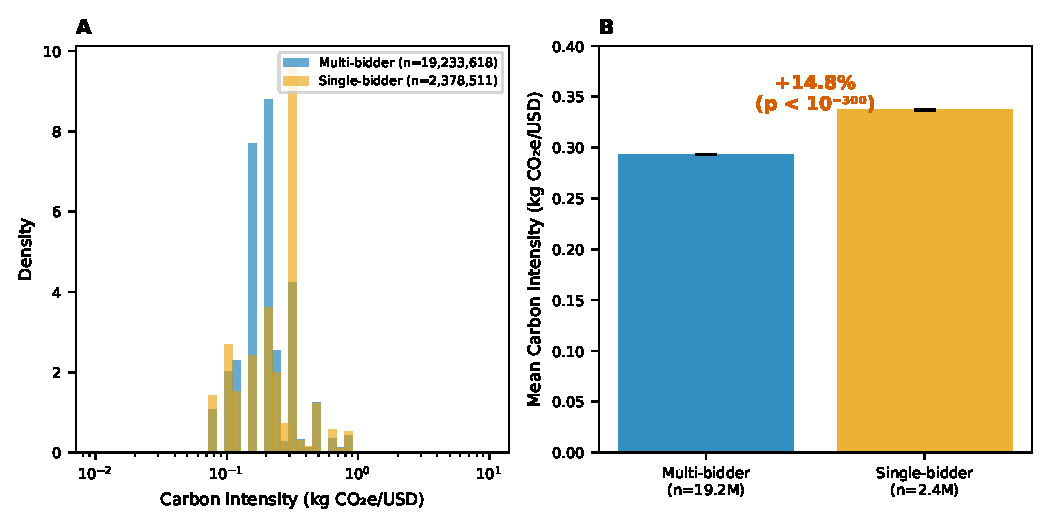
\includegraphics[width=0.95\textwidth]{Fig1_competition_carbon.pdf}
\caption{\textbf{Governance-contingent carbon-competition gap across 27 countries (2012--2023).} (\textbf{A}) Mean single-bidder carbon premium (\%) by governance quality quartile (World Bank WGI composite score\cite{worldbank2023wgi}). EU-context countries (top governance quartile) show a $-4.3\%$ negative premium: governance has pushed competition into the highest-carbon sectors. Cross-country heterogeneity is $I^2 = 99.3\%$. (\textbf{B}) Portfolio carbon intensity premium (\%) by contract scale across all 27 countries. The global pattern (influenced by Colombia's composition effect) shows $+50.2\%$ for small contracts and $-7.1\%$ for large; within EU-context countries, the premium is negative across all scales ($-2.8\%$ to $-7.8\%$; Table~\ref{tab:ucurve}). Confidence intervals are 95\% (clustered by country). $N = 21{,}612{,}129$ contracts.}
\label{fig:carbon_competition}
\end{figure}

\begin{figure}[H]
\centering
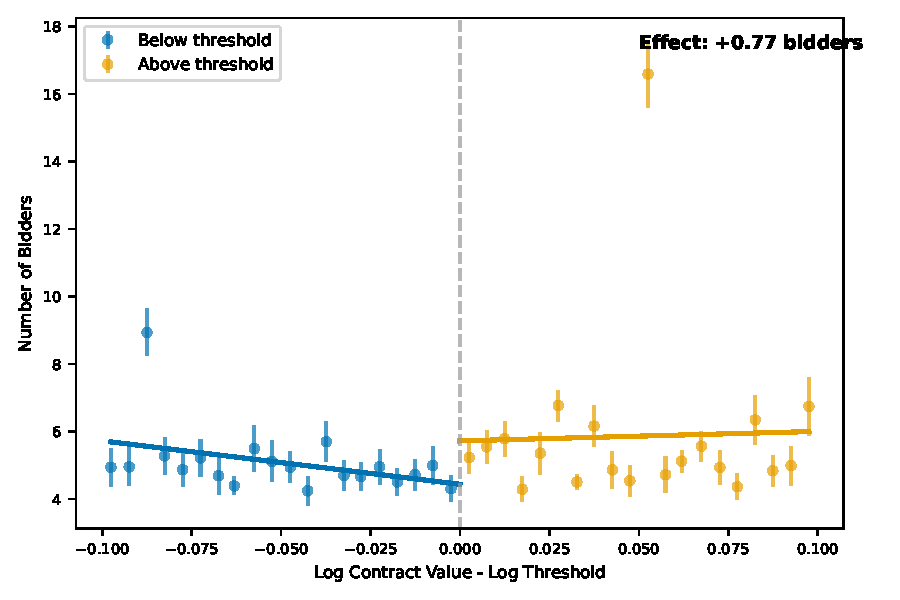
\includegraphics[width=0.95\textwidth]{Fig2_rdd_competition.pdf}
\caption{\textbf{Decarbonization Dead Zones, EU reform DiD, and post-pandemic single-bidder trends.} (\textbf{A}) Bubble chart of procurement sectors positioned by carbon intensity (x-axis) and single-bidder rate (y-axis); bubble area represents total contract value. The shaded upper-right quadrant marks the strict EU-context Dead Zone screen; the global 22-sector Dead Zone classification contains an estimated \texteuro190--250 billion annually in single-bidder contracts after OECD calibration (database-reported values are ${\sim}7\times$ higher due to framework-agreement maximum amounts; see Methods). (\textbf{B}) Annual single-bidder rates for treated EU countries (solid) vs. Norway/Switzerland comparators (dashed), 2012--2023. Vertical lines mark EU Directive transposition (April 2016) and e-procurement mandate (October 2018, $-0.8$ pp discontinuity). The primary staggered group-time specification yields ATT $= -7.2$ pp (RMSPE permutation $p = 0.042$; effect-magnitude permutation $p = 0.174$; see Methods); conventional TWFE is attenuated and imprecise ($-0.71$ pp, $p = 0.57$). (\textbf{C}) EU-context single-bidder rates by year: 16.1\% (2019), 15.4\% (2020, acute pandemic), rising to 18.6\% (2023), a $+2.5$ pp increase whose causal mechanism requires further investigation.}
\label{fig:rd_competition}
\end{figure}

\begin{figure}[H]
\centering
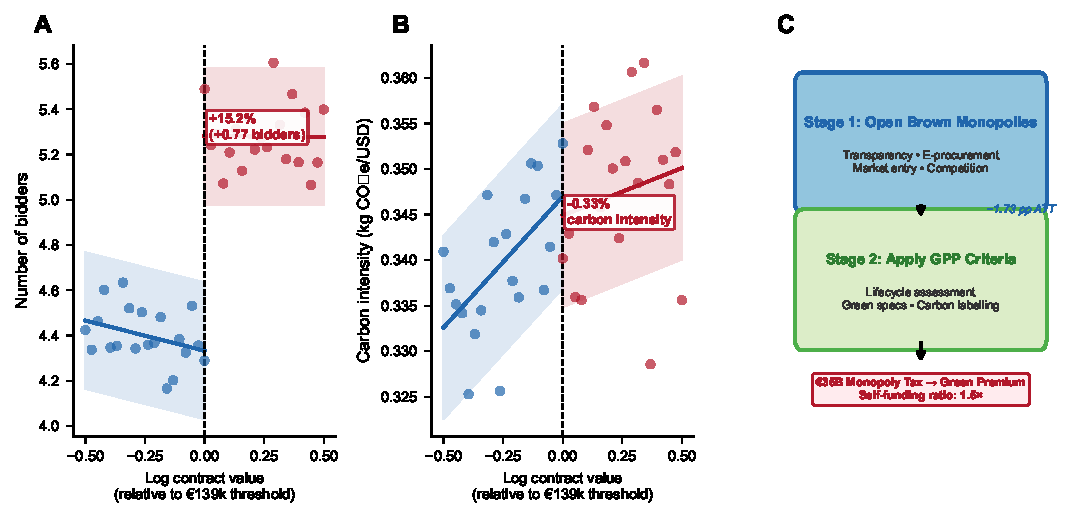
\includegraphics[width=0.95\textwidth]{Fig3_counterfactual.pdf}
\caption{\textbf{Causal evidence from local-linear regression discontinuity design at the EU transparency cutoff.} (\textbf{A}) Number of bidders as a function of log contract value relative to the \texteuro139,000 EU threshold (binned visualization; $N = 553{,}293$ contracts with observed bidder counts within $\pm 0.10$ log-EUR). A local-linear RDD (triangular kernel, HC2 SE) estimates $\hat{\tau} = +0.32$ additional bidders at the cutoff ($p < 0.001$); under the MSE-optimal bandwidth ($h^* = 0.067$, $N = 380{,}938$), $\hat{\tau} = +0.15$ ($p = 0.029$). Sign-stable across all 26 bandwidth specifications ($h \in [0.05, 0.30]$); 25/26 significant at $p < 0.05$. Density-ratio stability test: density ratio (above/below) $= 1.12$ at $\pm 0.10$ log-EUR vs.\ $1.48$ at $\pm 0.50$ --- ratio \emph{decreases} toward the cutoff, the opposite of a manipulation spike; 15.5\% raw count asymmetry reflects voluntary-disclosure composition (SI \S4). (\textbf{B}) Carbon intensity (kg CO$_2$e/USD) by contract value around the same threshold. The RDD carbon effect is positive at the MSE-optimal bandwidth ($\hat{\tau} = +0.006$ kg/USD; $t = 3.74$; $p < 0.001$) but mixed in sign across the sensitivity grid (19/26 bandwidths negative), indicating a bandwidth-sensitive compositional shift at the threshold. (\textbf{C}) Schematic of the two-stage governance-first GPP architecture: Stage 1 (transparency reform opens Dead Zone competition) enables Stage 2 (GPP criteria effective within newly competitive markets).}
\label{fig:counterfactual}
\end{figure}

\begin{figure}[H]
\centering
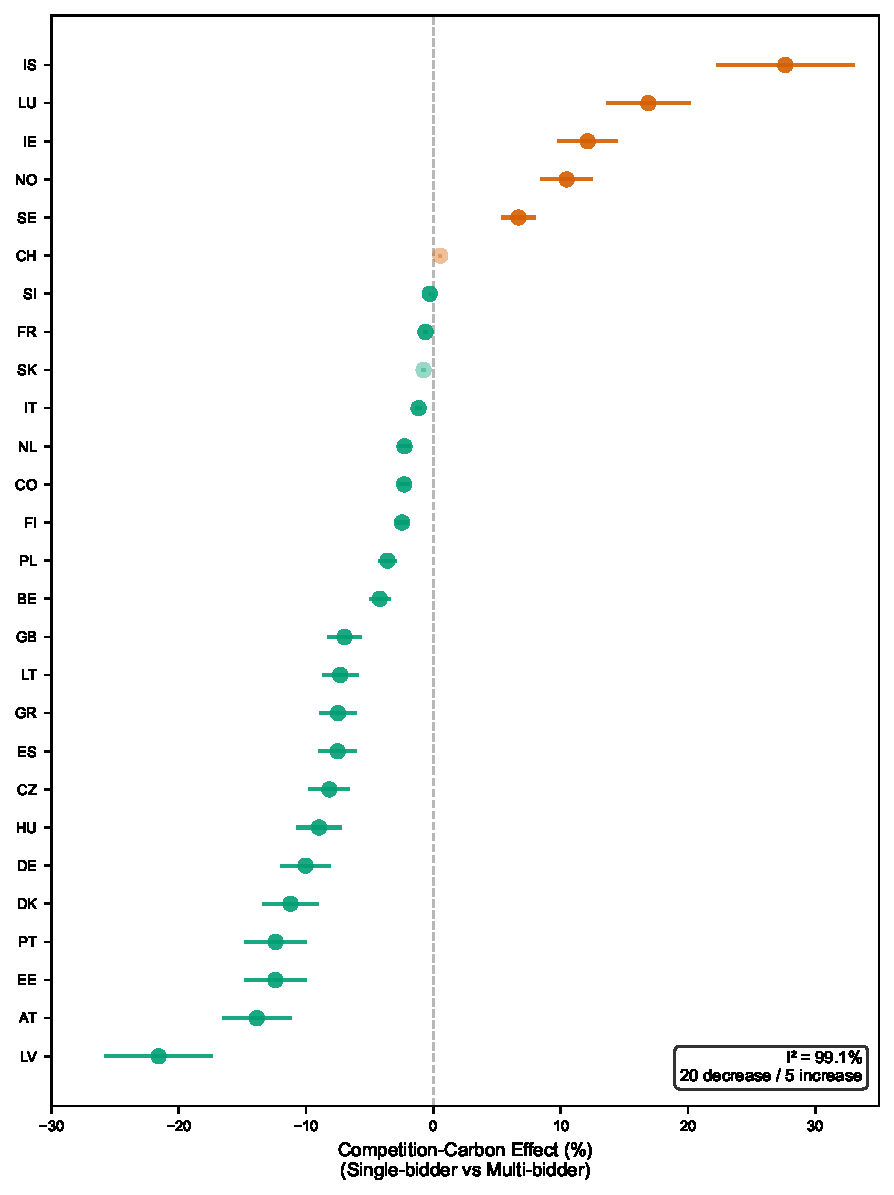
\includegraphics[width=0.95\textwidth]{Fig4_country_forest.pdf}
\caption{\textbf{Country-level DiD effects: heterogeneity in governance reform impact.} Forest plot of country-specific single-bidder rate changes following Directive 2014/24/EU transposition across 25 countries (23 EU member states plus Norway and Switzerland as never-treated EEA/EFTA comparators). Effect sizes are estimated via the Callaway \& Sant'Anna (2021) group-time estimator; bars show 95\% confidence intervals. The aggregate ATT is $-7.2$ pp (RMSPE permutation $p = 0.042$). After an imprecise first post-treatment year, the 2016 cohort (13 countries) shows large reductions from the second post-treatment year onward ($-5.5$ to $-10.3$ pp in later post-treatment years); the 2017 cohort shows a smaller initial effect that attenuates toward zero by 2023, consistent with less reform-intensive transposition. This country-level heterogeneity is the primary driver of TWFE attenuation under the pooled specification (SI Table~S14). Norway (NO) and Switzerland (CH) serve as never-treated comparators and are shown for reference.}
\label{fig:country_forest}
\end{figure}
\end{document}
